\newpage
\subsection{Back-end}

Nella parte back-end sono presenti i package \textit{Gateway} e \textit{Services} strutturati secondo un'architettura a microservizi, i quali hanno una dipendenza verso l'interfaccia \textit{serviceInteractionHandler}.

\begin{figure}[H]
	\centering
	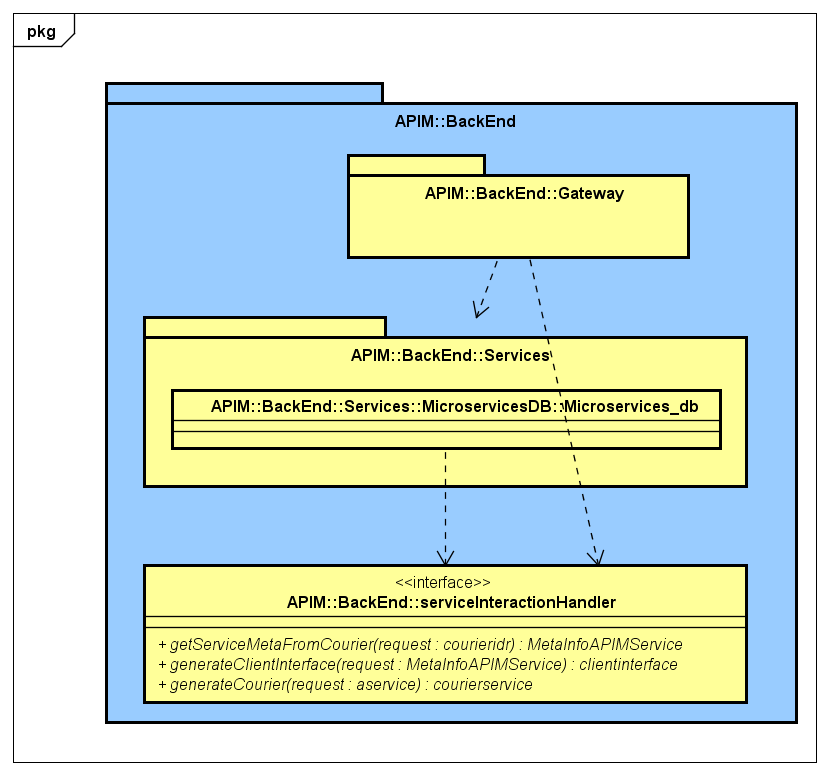
\includegraphics
	[width=0.7\linewidth]
	{UML/DiagrammiPackage/BackEnd.png}
	\caption{Package APIM::BackEnd}
\end{figure}

\begin{itemize}
	\item \textbf{Padre}: APIM;
	
	\item \textbf{Descrizione}: package contenente le componenti del back-end dell'applicazione;
	
	\item \textbf{Package contenuti}:
	\begin{itemize}
		\item \textbf{\textit{Gateway}}: package contenente le classi e le interfacce per il funzionamento dell'API Gateway;
		
		\item \textbf{\textit{Services}}: package contenente tutti i microservizi per le comunicazioni con i database.
	\end{itemize}
	\item \textbf{Classi contenute}:
		\begin{itemize}
			\item \textbf{\textit{serviceInteractionHandler}}: interfaccia per la gestione delle comunicazioni dell'API Gateway e dei \textit{services}.
		\end{itemize}
\end{itemize}

\subsubsection{Gateway}
\begin{figure}[H]
	\centering
	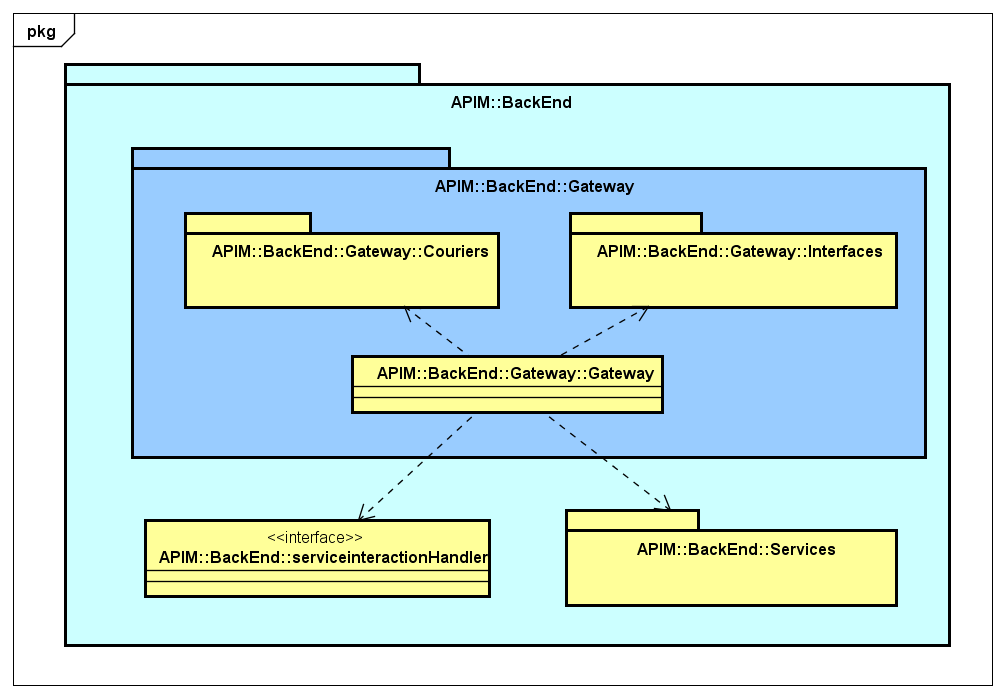
\includegraphics
	[width=0.7\linewidth]
	{UML/DiagrammiPackage/gateway.png}
	\caption{Package APIM::BackEnd::Gateway}
\end{figure}

\begin{itemize}
	\item \textbf{Padre}: BackEnd;
	
	\item \textbf{Descrizione}: package contenente la componente principale del lato back-end. Pur essendo integrato nella sistema, è un modulo che svolge funzioni separate alla piattaforma vera e propria: infatti, l'API Gateway si occupa di controllare e reindirizzare le chiamate effettuate dai clienti ai microservizi (prodotti) inseriti nel marketplace \progetto, verificandone la validità (credenziali, chiave) e monitorandone l'uso (SLA, utilizzi rimanenti).
	
	\item \textbf{Relazioni d'uso con altri componenti}: la classe \textit{Gateway} comunica con le classi contenute all'interno del package \textit{Services}. Inoltre, necessita delle interfacce contenute nel package \textit{Interfaces} e crea le sessioni \textit{couriers} Jolie, archiviandole nel package \textit{Couriers}.
	
	\item \textbf{Package contenuti}:
	\begin{itemize}
		\item \textbf{\textit{Couriers}}: package contenente l'archivio delle sessioni couriers dei microservizi Jolie. Le sessioni couriers vengono create dal gateway ed utilizzate da \textit{serviceinteractionhandler}. Inoltr, forniscono i dati necessari al funzionamento del package \textit{Interfaces}.\\
		Le sessioni couriers permettono l'overloading dei messaggi inviati nelle chiamate dei microservizi al gateway, così da allegare alla richiesta le informazioni per raggiungere il microservizio desiderato.
		
		\item \textbf{\textit{Interfaces}}: package contenente le interfacce necessarie al funzionamento dell'API Gateway. Si occupa dei dati riguardanti le chiamate ai microservizi, in particolar modo, il tipo di operazione richiesta e le informazioni riguardanti l'interfaccia del microservizio target.
	\end{itemize}
	\item \textbf{Classi contenute}:
		\begin{itemize}
			\item \textbf{\textit{Gateway}}: classe che rappresenta la struttura dell'API Gateway della piattaforma \progetto.
		\end{itemize}
\end{itemize}

\subsubsection{Services}
Tale package contiene tutti i servizi appartenenti al lato back-end della piattaforma, eccezion fatta per il gateway già descritto nella sezione soprastante. \textit{Services} contiene tutte le classi di comunicazione con i database che permetteranno il corretto funzionamento dell'applicazione.

\begin{figure}[H]
	\centering
	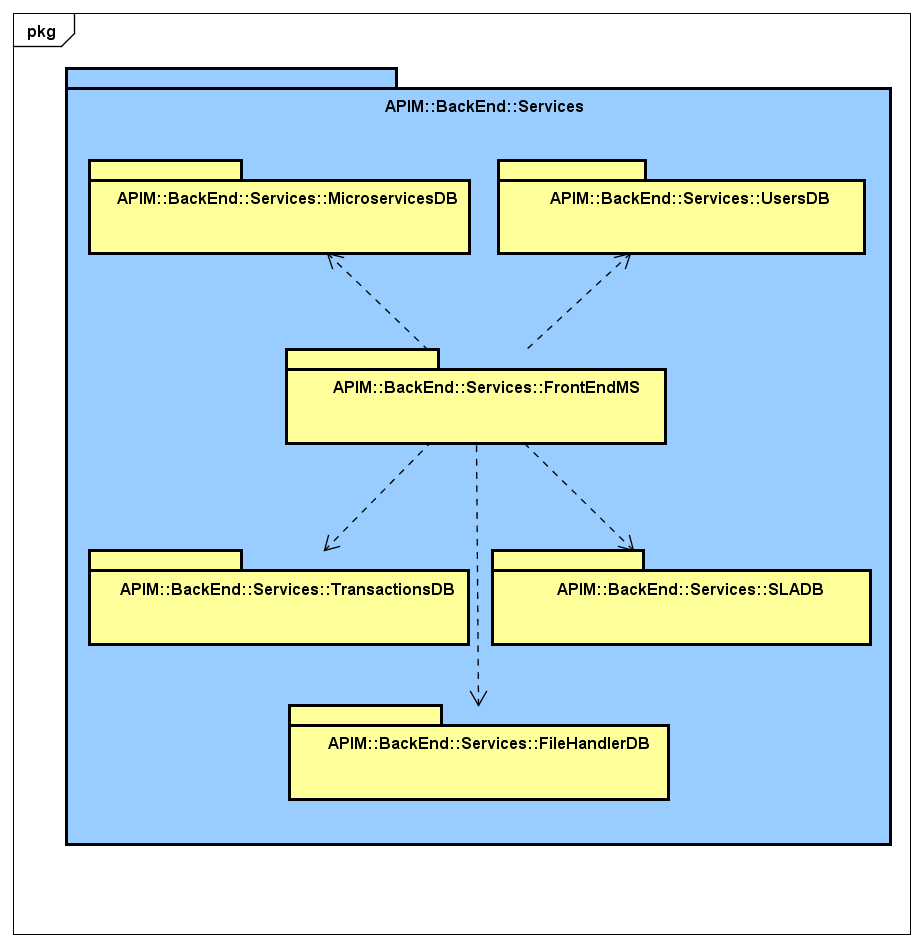
\includegraphics
	[width=0.7\linewidth]
	{UML/DiagrammiPackage/services.png}
	\caption{Package APIM::BackEnd::Services}
\end{figure}

\begin{itemize}
	\item \textbf{Padre}: BackEnd;
	
	\item \textbf{Descrizione}: package che contiene tutti i package relativi ai microservizi del back-end dell'applicazione;
	
	\item \textbf{Relazioni d'uso con altri componenti}: questo package si relaziona con l'API Gateway;
	
	\item \textbf{Package contenuti}:
	\begin{itemize}
		\item \textbf{\textit{UsersDB}}: package contenente le classi che permettono la comunicazione con il database relativo agli utenti del sistema;
		
		\item \textbf{\textit{MicroservicesDB}}: package contenente le classi che permettono la comunicazione con il database relativo ai microservizi registrati sulla piattaforma;
		
		\item \textbf{\textit{TransactionsDB}}: package contenente le classi che permettono la comunicazione con il database relativo alle transazioni degli utenti del sistema;
		
		\item \textbf{\textit{SLADB}}: package contenente le classi che permettono la comunicazione con il database relativo alle informazioni di SLA dei microservizi utilizzati tramite l'API Gateway della piattaforma \progetto;
		
		\item \textbf{\textit{FileHandlerDB}}: package contenente le classi che permettono la gestione dei file;
		
		\item \textbf{\textit{FrontEndMS}}: package contenente le classi che si occupano delle operazioni più complesse, quali l'accesso a più di un database.
	\end{itemize}
\end{itemize}

\paragraph{UsersDB}

\begin{figure}[H]
	\centering
	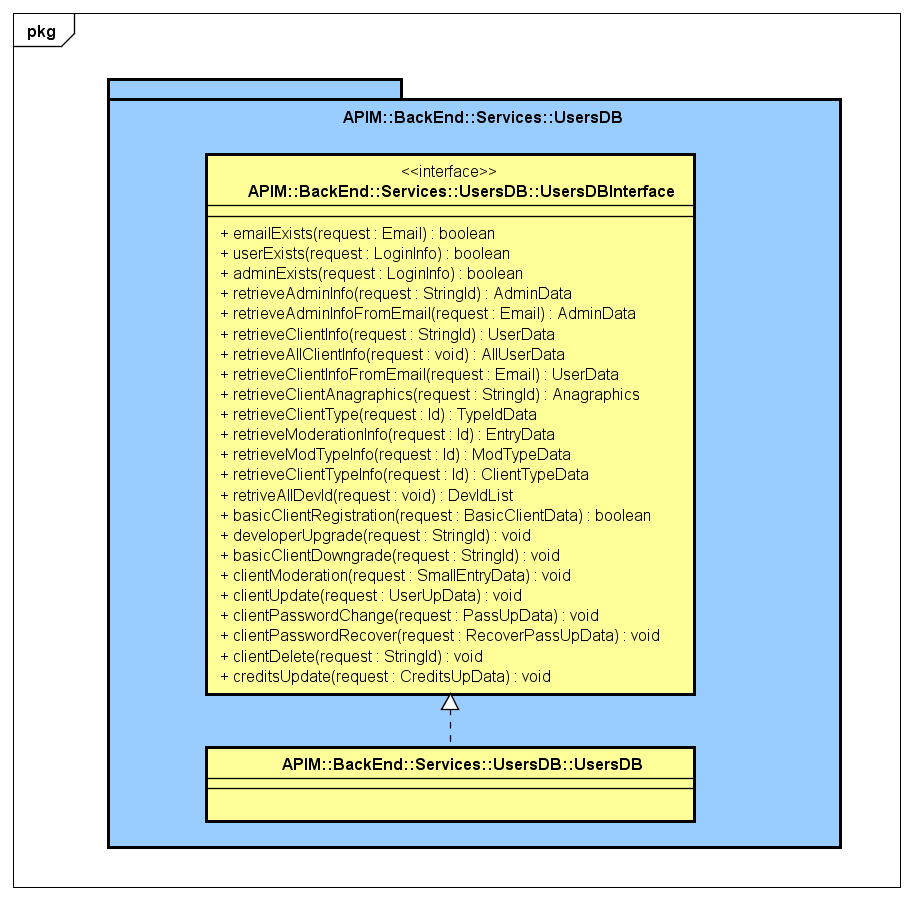
\includegraphics
	[width=0.7\linewidth]
	{UML/DiagrammiPackage/UsersDB.png}
	\caption{Package APIM::BackEnd::Services::UsersDB}
\end{figure}

\begin{itemize}
	\item \textbf{Padre}: Services;
	
	\item \textbf{Descrizione}: package che contiene le classi di comunicazione con il database dell'applicazione relativo alle informazioni (anagrafiche e personali) degli utenti (admin, clienti, sviluppatori) del sistema;
	
	\item \textbf{Relazioni d'uso con altri componenti}: questo package si relaziona con il sub-package \textit{FrontEndMS} del package padre, fornendogli i dati che esso richiede riguardo alle operazioni con il database delle informazioni degli utenti;
	
	\item \textbf{Classi contenute}:
		\begin{itemize}
			\item \textbf{\textit{Users\_dbInterface}}: interfaccia che raccoglie tutte le \textit{operation} riguardanti il database degli utenti;
			
			\item \textbf{\textit{Users\_db}}: classe che implementa l'interfaccia \textit{Users\_dbInterface}.
		\end{itemize}
\end{itemize}

\paragraph{MicroservicesDB}

\begin{figure}[H]
	\centering
	\includegraphics
	[width=0.7\linewidth]
	{UML/DiagrammiPackage/MicroservicesDB.png}
	\caption{Package APIM::BackEnd::Services::MicroservicesDB}
\end{figure}

\begin{itemize}
	\item \textbf{Padre}: Services;
	
	\item \textbf{Descrizione}: package che contiene le classi di comunicazione con il database dell'applicazione relativo ai microservizi registrati nella piattaforma;
	
	\item \textbf{Relazioni d'uso con altri componenti}: questo package si relaziona con il package \textit{FrontendMS}, fornendogli i dati che esso richiede riguardo alle operazioni con il database delle informazioni dei microservizi.\\
	Inoltre, comunica con il Gateway per permettere l'identificazione e l'utilizzo dei microservizi, e garantire correttezza, efficienza e validità delle chiamate;
	
	\item \textbf{Classi contenute}:
	\begin{itemize}
		\item \textbf{\textit{Microservices\_dbInterface}}: interfaccia che raccoglie tutte le \textit{operation} riguardanti il database dei microservizi;
		
		\item \textbf{\textit{Microservices\_db}}: classe che implementa le interfacce \textit{Microservices\_dbInterface} e \textit{serviceInteractionHandler}.
	\end{itemize}
\end{itemize}

\paragraph{TransactionsDB}

\begin{figure}[H]
	\centering
	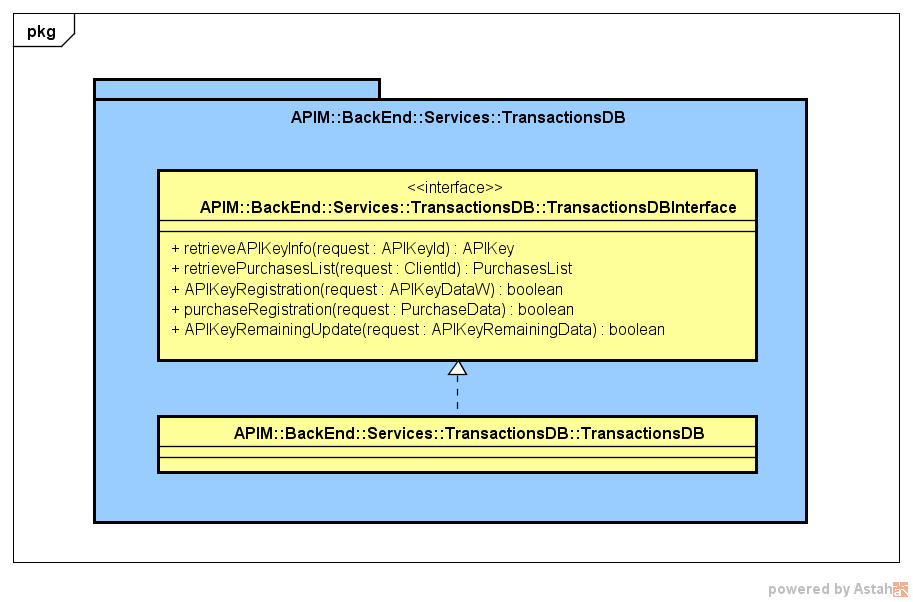
\includegraphics
	[width=0.7\linewidth]
	{UML/DiagrammiPackage/TransactionsDB.png}
	\caption{Package APIM::BackEnd::Services::TransactionsDB}
\end{figure}

\begin{itemize}
	\item \textbf{Padre}: Services;
	
	\item \textbf{Descrizione}: package che contiene le classi di comunicazione con il database dell'applicazione che si occupa di immagazzinare i dati sulle transazioni;
	
	\item \textbf{Relazioni d'uso con altri componenti}: questo package si relaziona con il package \textit{FrontendMS}, fornendogli i dati che esso richiede riguardo alle operazioni con il database delle informazioni delle transazioni.\\
	Comunica inoltre con il Gateway per verificare la validità delle API Key e/o aggiornare i dati relativi (usi residui della chiave) alle chiamate ai microservizi effettuate;
	
	\item \textbf{Classi contenute}:
	\begin{itemize}
		\item \textbf{\textit{Transactions\_dbInterface}}: interfaccia che raccoglie tutte le \textit{operation} riguardanti il database delle transazioni;
		
		\item \textbf{\textit{Transactions\_db}}: classe che implementa l'interfaccia \textit{Transactions\_dbInterface}.
	\end{itemize}
\end{itemize}

\paragraph{SLADB}

\begin{figure}[H]
	\centering
	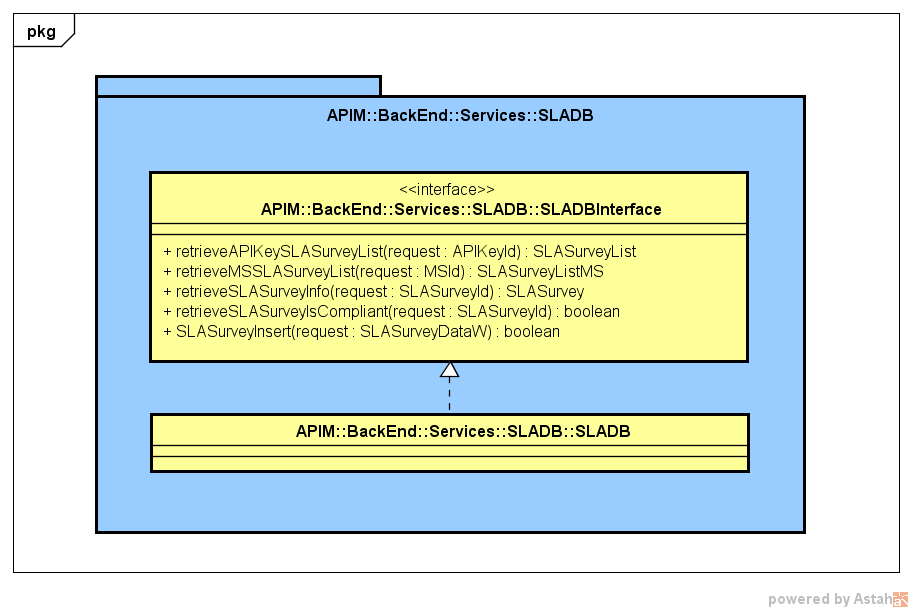
\includegraphics
	[width=0.7\linewidth]
	{UML/DiagrammiPackage/SLADB.png}
	\caption{Package APIM::BackEnd::Services::SLADB}
\end{figure}

\begin{itemize}
	\item \textbf{Padre}: Services;
	
	\item \textbf{Descrizione}: package che contiene le classi di comunicazione con il database che si occupa di immagazzinare e trattare i dati relativi al Service Level Agreement (SLA);
	
	\item \textbf{Relazioni d'uso con altri componenti}: questo package si relaziona con il package \textit{FrontendMS}, fornendogli i dati che esso richiede riguardo alle operazioni con il database delle informazioni della SLA.\\
	Inoltre, comunica con il Gateway per aggiornare i dati delle performance di risposta di ogni microservizio utilizzato;
	
	\item \textbf{Classi contenute}:
	\begin{itemize}
		\item \textbf{\textit{SLA\_dbInterface}}: interfaccia che raccoglie tutte le \textit{operation} riguardanti il database delle informazioni di SLA;
		
		\item \textbf{\textit{SLA\_db}}: classe che implementa l'interfaccia \textit{SLA\_dbInterface}.
	\end{itemize}
\end{itemize}

\paragraph{FileHandlerDB}

\begin{figure}[H]
	\centering
	\includegraphics
	[width=0.7\linewidth]
	{UML/DiagrammiPackage/FileHandlerDB.png}
	\caption{Package APIM::BackEnd::Services::FileHandlerDB}
\end{figure}

\begin{itemize}
	\item \textbf{Padre}: Services;
	
	\item \textbf{Descrizione}: package che si occupa della gestione dei file, e presenta le classi di comunicazione con il database per tale finalità;
	
	\item \textbf{Relazioni d'uso con altri componenti}: questo package si relaziona con il package \textit{FrontendMS}, fornendogli i dati che esso richiede riguardo alle operazioni con il database delle informazioni dei file.\\
	Inoltre, comunica con il Gateway per recuperare i file legati alle interfacce dei microservizi;
	
	\item \textbf{Classi contenute}:
	\begin{itemize}
		\item \textbf{\textit{FileHandlerInterface}}: interfaccia che raccoglie tutte le \textit{operation} riguardanti la gestione dei file;
		
		\item \textbf{\textit{FileHandler}}: classe che implementa l'interfaccia \textit{FileHandlerInterface}.
	\end{itemize}
\end{itemize}
